\chapter{Methods in ...}

\section{Introduction of method}
In this chapter the setup of Husky and TB3 both hardware and software will be explained. Then how both where setup to drive autonomous independently. Lastly the platooning algorithms will be explained. 


Before getting into the setup of Husky and TB3 it is necessary to explain the the custom packages made for this project $masteruia$ \cite{masteruia} and $uia\_husky\_0776$ \cite{uiahusky}. 

There where three project on the Husky at the same time, so a common GitHub was made $uia\_husky\_0776$. All the software used by the Husky in this project is included in $uia\_husky\_0776$ such as packages for Husky, OS1, UM7 and "pointcloud\_to\_laserscan".

$masteruia$ is the other GitHub used in the project and contains two packages $uia\_husky\_0776$ and $tb3\_cpp$.
First off the folder called $uia\_husky\_0776$ is a copy of the one talked about above. The folder was made when trying to launch the Husky with namespace, this task was not completed. 
The $tb3\_cpp$ is standard ROS2 CMake package consisting a launch file for TB3, nodes for Nav2 API and platooning algorithm. 
                      

\section{Husky}
\subsection{Hardware}
This section will describe the setup of the Husky and its components. 

The IMU was glued to the center of the tray, connected with a USB to the Xavier. 
In the Husky there are two Xavier only one of them is used in this project. The one used is Xavier1 the other is Xavier2. Both of the Xaviers where placed in the tray and secured with a 3D printed mount. The Xaviers where lacking USB ports so both of them got a USB hub. 
The Ouster LiDAR has two components the laser scanner and the power/data brick. The scanner is mounted on top of a aluminum frame in the front for long distance scanning. The brick is blued to the front wall off the tray, connected to 24 volt barrel jack and Ethernet form the router. 
The router is mounted in the front of the aluminum frame powered by 12 volt barrel jack. Xavier and Xavier2 is connected with Ethernet, Xavier also has a WiFi connection. 
\begin{figure}[H]
  \centering
  \begin{minipage}[b]{0.4\textwidth}
    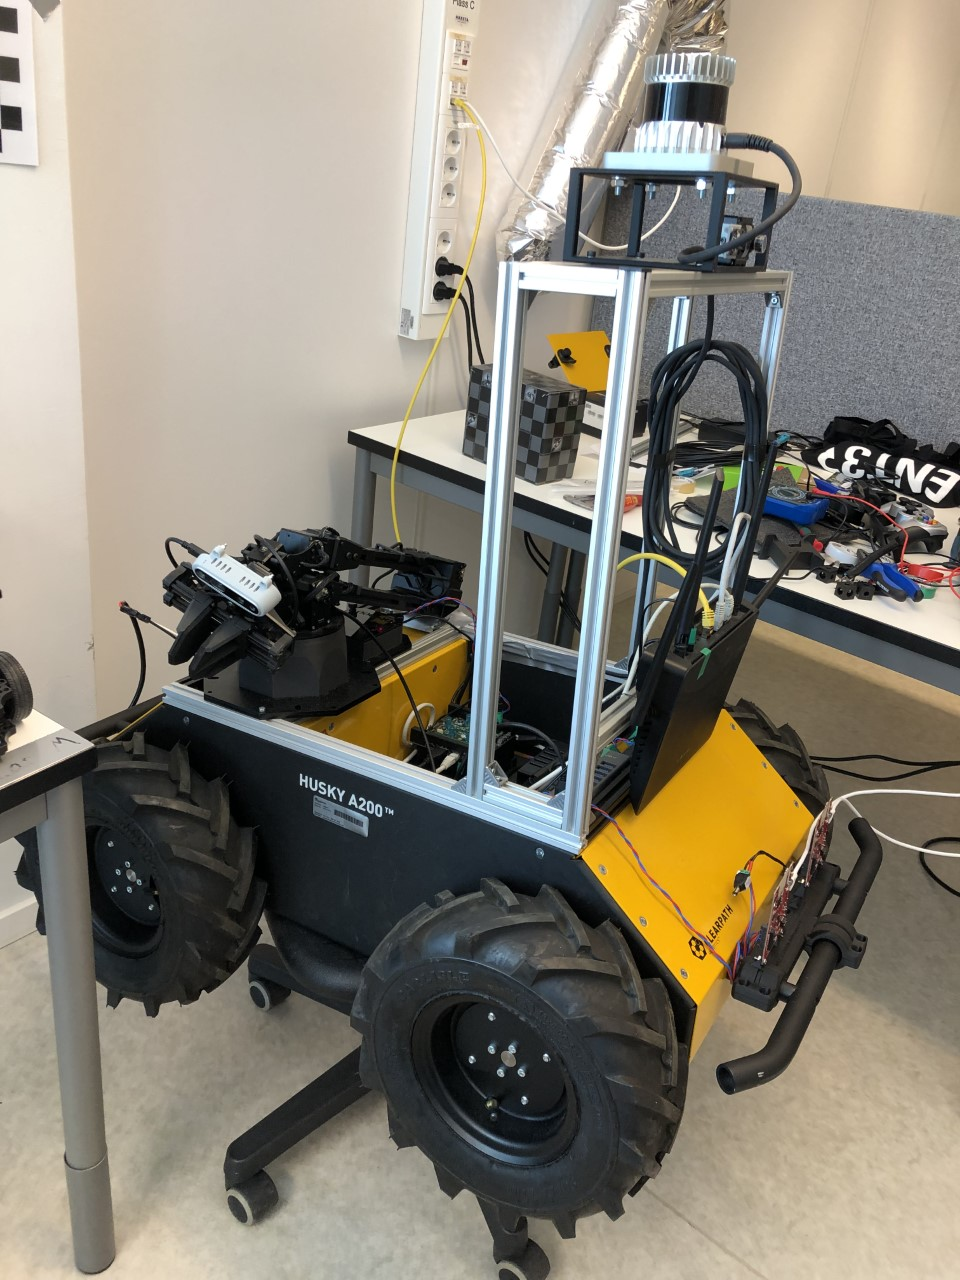
\includegraphics[width=\textwidth]{Figures/images/husky_irl.jpg}
    \caption{Photo of Husky}
    \label{fig:husky_irl}
  \end{minipage}
  \hfill
  \begin{minipage}[b]{0.59\textwidth}
    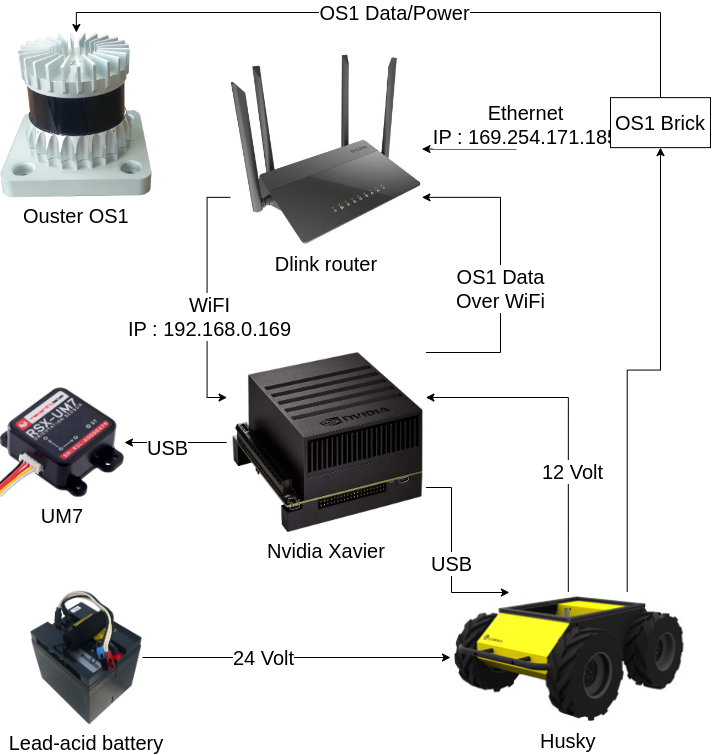
\includegraphics[width=\textwidth]{Figures/drawio/Husky_HW.drawio.png}
    \caption{Husky hardware map, this dose not include components on the Husky used in other projects}
    \label{fig:Husky_HW}
  \end{minipage}
\end{figure}

\subsection{Software}
This section will describe thee setup of the Husky without Nav2, the "base" setup of the Husky. For less comfusion all \topic{topics} and \node{nodes} have colors and there ROS2 name 
The Xavier1 on the Husky is runnning Ubuntu 20.04 Desktop \cite{ubuntu20_04} with ROS2 foxy \cite{rosfoxyinstall} and galactic \cite{rosgalacticinstall}, Nav2 binary \cite{rosnavinstall}, Husky foxy Debian packages \cite{huskyinstall} and $uia\_husky\_0776$ \cite{uiahusky}. When setting up the ROS2 software Rviz and rqt was used to test all components. 


$uia\_husky\_0776$ includes packages for Husky, OS1, UM7 and $pointcloud\_to\_laserscan$. A launch file was made to launch it all at once "husky.launch.py" in "uia\_husky\_0776/husky\_group/launch/".


Clearpath provides binary packages for the Husky in ROS2 foxy, because of this the hole project was set up foxy in the beginning . The Clearpath packages provides the essential software for making the husky move with ROS2.

An other project on the Husky was pick and place and used the ViperX 300 Robot Arm. This arm was better to set up with Galactic, so the project was converted to Galactic. Foxy and Galactic are similar and didn't cause any issues, except for with the Husky package. Clearpath did not provide binary packages for the Husky in Galactic just source. This source files did not initially work on the Husky. The student working on pick and place made some changes to the source files, making them work. Still the source files on Galactic are more unstable then Foxy. Therefor "base\_launch.py" is launched in Foxy and the rest of the project in Galactic. 

The Husky is launched with the $husky.launch.py$ from $husky\_group$ in the $uia\_husky\_0776$. $husky.launch.py$ pass in parameters and starts $base\_launch.py$, \node{um7\_node}, $os1_launch.py$ and \node{pointcloud\_to\_laserscan}. 

$base\_launch.py$ starts up the /joy\_teleop and /robot\_state system and the nodes \node{/twist\_mux}, \node{/huksy\_velocity\_controller} and \node{/ekf\_node}. 

\begin{itemize}
    \item joy\_teleop system converts a Logitech joystick controllers signal into \topic{joy\_teleop/cmd\_vel} a standard velocity massage with namespace. 
    
    \item \node{/twist\_mux} converts \topic{/cmd\_vel} with and without namespaces to \topic{/husky\_velocity\_controller/cmd\_vel\_unstamped} and sends it into \node{/huksy\_velocity\_controller}. Every velocity command for the Husky goes though the \node{/twist\_mux}, joystick, keyboard and Nav2. 
    
    \item \node{/huksy\_velocity\_controller} controlles the motors and publishes \topic{/odom} based on the wheel encounters on the Husky. 
    
    \item \node{/ekf\_node} fuses odometry(\topic{/odom}) and IMU(\topic{/imu/data}) to \topic{"/odometry/filtered"} to localize the Husky with greater precision[need a cite?]. 
    
    \item The /robot\_state system combines the URDF with the joint state of the wheels to create a accurate model of the Husky in Rviz. 
    
\end{itemize}

The UM7 ROS2 package where found on GitHub \cite{um7imu}. This packages launches a node called \node{/um7\_dirver} publishing data from the IMU on topic \topic{/imu/data}, into \node{/ekf\_node}.
\\ \newline
Ouster has a well documented GitHub \cite{ousterros} with ROS2 drivers for there hardware, including the OS1. The package starts up a node called \node{/ouster\_driver} witch publishes \topic{/points}. 
Since Nav2 uses \topic{/scan} as perception topic, a packages called "pointcloud\_to\_laserscan" \cite{pcl2laser} was installed to make the OS1 communicate with Nav2. "pointcloud\_to\_laserscan" was also found on GitHub . 

This image represents software of the Husky in a rqt format where 
ovals are \node{nodes} and squares is \topic{topics}. This dose not include Nav2. The original rqt image can be found here \ref{Appendix:HuskySWmap}. 

\begin{figure}[H]
    \centering
    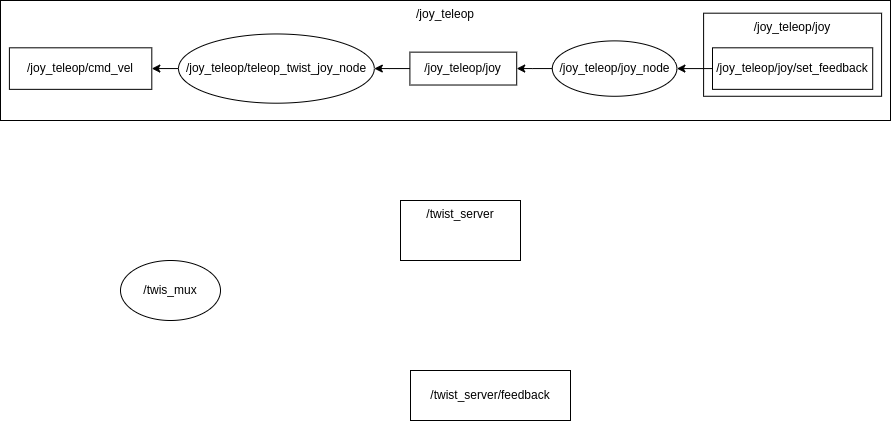
\includegraphics[width = 1\textwidth]{Figures/drawio/husky_rqt.drawio.png}
    \caption{Husky software map}
    \label{fig:HuskySW}
\end{figure}

\section{TurtleBot3}
\subsection{Hardware}
The TurtleBot3 started with no battery and was driven by a Raspberry Pi. The Pi was running Ubuntu Server and had an old student project saved. It had performance issues, writing in the TUI was choppy. The Pi was flashed with Ubuntu Server 20.04 in an attempt to increase the performance. This did not work, and therefor it was decided tho switch out the Pi. A Xavier was available, it is same as the Husky is using and was therefor chosen. The TurtleBot3 uses a battery similar to RC Cars, RC battery's was ordered though a local hobby store. Figure \ref{fig:TB3Hardware} shows the map of the TB3 hardware. 

\begin{figure}[H]
    \centering
    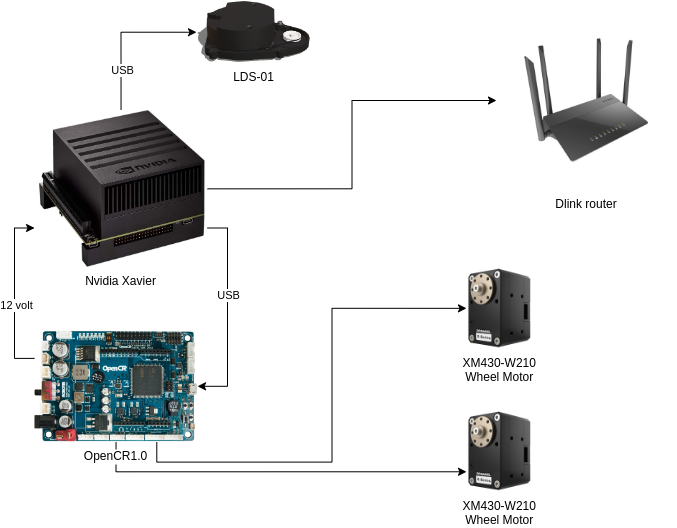
\includegraphics[width = 0.5\textwidth]{Figures/drawio/TB_HW.drawio.png}
    \caption{TurtleBot3 hardware map}
    \label{fig:TB3Hardware}
\end{figure}

\subsection{Software}

This will describe the setup of the TB3 without Nav2, the "base" setup TB3.  
The name of user on the TB3 Xavier is tb and will be the reference. tb is running Ubuntu 20.04 Desktop \cite{ubuntu20_04} with ROS2 galactic Debian(binary) \cite{rosgalacticinstall}, TB3 packages binary \cite{turtlebot3galactic}, Nav2 binary \cite{rosnavinstall} and $masteruia$ \cite{masteruia}. For practical reasons a custom launch file was made for the TB3 in the $masteruia$ package. 

The "robot.launch.py" from the TB3 packages is the file used for launch the TB3 in this project. "robot.launch.py" bring up four nodes \node{/turtlebot3\_node}, \node{/hlds\_laser\_publisher}, \node{/robot\_state\_publisher} and \node{/diff\_drive\_controller}. 
\node{/hlds\_laser\_publisher} starts up LDS1.0 and publishes the LiDAR data on the \topic{/scan} topic. \node{/turtlebot3\_node} publishes five topics and subscribes to one. It subscribes to to \topic{/cmd\_vel} converts it to wheel position and publishes \topic{/joint\_states}. The raw IMU data is picked up by the \node{turtlebot3\_node} and published on the ROS network under \topic{/imu} topic. \topic{/magnetic\_field}, \topic{sensor\_state} and \topic{/battery\_state} are not used in this project. 
\node{/diff\_drive\_controller} fuses \topic{/imu} and \topic{/joint\_states} and publish the fused odometry under \topic{/odom}. 
\node{/robot\_state\_publisher} combines the URDF and \topic{/joint\_states} for a complete description of the TB3 under \topic{/robot\_description}.

\begin{figure}[H]
    \centering
    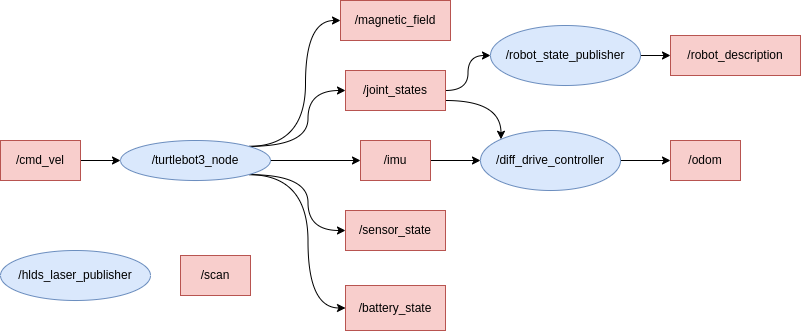
\includegraphics[width = 1\textwidth]{Figures/drawio/TB3_rqt.drawio.png}
    \caption{TurtleBot3 software map}
    \label{fig:TB3SW}
\end{figure}

To achieve namespace like in Figure \ref{fig:TB3SW} $tb3\_cpp$ package was made in the $masteruia$ GitHub \cite{masteruia}. This contains three folders launch, params and src. In launch the "tb3\_launch.py" is the only one used the rest is leftovers from working. "tb3\_launch.py" is  a launch file based on using the "robot.launch.py" from "turtlebot3\_bringup" \cite{turtlebot3galactic} to launch the TB3. Here is how it works in order: 
\begin{enumerate}
\item Exporting "TURTLEBOT3\_MODEL" is required by "robot.launch.py" 
\item Opens access to LiDAR and OpenCR1.0 
\item Pushing namespace to TB3 
\item Finding and executing standard TB3 launch
\item Passing in custom parameters file for to add namespace to all the nodes 
\end{enumerate}  

The "params" folder is full of work leftovers except for "tb3\_param.yaml" witch is a copy of the standard TB3 waffle parameter file with "tb:" added in front of the nodes for namespacing.

Last folder "src" contains nodes from this project. "cmd\_vel\_subpub\_v1.py is the algorithm Time Delay \ref{Platooning_algorithm}. "feedback.py", "nav2.py", "pose\_pub\_v*.py" and "pose\_sub\_v*.py" is nodes used when attempting to use Nav2 API for a platooning algorithm \ref{Platooning_algorithm}.

\section{Autonomous driving on Husky and TB3 independently}
Both robots where set up to drive autonomous and is able to do so independently. In the beginning it was thought this was necessary to archive autonomous platooning. There where two ways the robots could drive autonomous with and without a pre made map. 

Driving with simultaneous localization and mapping (SLAM) , and navigation or without a pre made map. First the base of the robot is launched, then SLAM lastly navigation. There are multiple ways of launching SLAM: 
\begin{lstlisting}[language=bash]
    ros2 launch slam_toolbox lifelong_launch.py 
    ros2 launch slam_toolbox online_async_launch.py
    ros2 launch slam_toolbox online_sync_launch.py
\end{lstlisting}
Read more about SLAM here \cite{slamtoolboxgithub}. All of the methods worked but "online\_async" was the most consistent and used. 

Here is how the Husky was launched to SLAM and navigate: 
Terminal 1: 
\begin{lstlisting}[language=bash]
    source /opt/ros/foxy/setup.bash
    source uia_husky_0776/install/local_setup.bash
    ros2 launch husky_group husky.launch.py
\end{lstlisting}
Terminal 2, note "use\_sim\_time:=false because" its not a simulation 
\begin{lstlisting}[language=bash]
    source /opt/ros/galactic/setup.bash
    ros2 launch slam_toolbox online_async_launch.py use_sim_time:=false
\end{lstlisting}
Terminal 3, note custom parameter file. 
\begin{lstlisting}[language=bash]
    source /opt/ros/galacitc/setup.bash
    ros2 launch nav2_bringup navigation_launch.py params_file:=uia_husky_0776/husky_group/params/nav2_params.yaml
\end{lstlisting}

The launch setup for the TB3 for SLAM and navigating at the same time: 
Terminal 1, note the "PushRosNamespace" where commented out in launch before this: 
\begin{lstlisting}[language=bash]
    source /opt/ros/galactic/setup.bash
    source masteruia/tb_ws/install/setup.bash
    ros2 launch tb3_cpp tb3_launch.py
\end{lstlisting}
Terminal 2, note "use\_sim\_time:=false because" its not a simulation 
\begin{lstlisting}[language=bash]
    source /opt/ros/galactic/setup.bash
    ros2 launch slam_toolbox online_async_launch.py use_sim_time:=false
\end{lstlisting}
Terminal 3, note custom parameter file. 
\begin{lstlisting}[language=bash]
    source /opt/ros/galacitc/setup.bash
    ros2 launch nav2_bringup navigation_launch.py 
\end{lstlisting}

Navigating with a pre made map uses the same setup for the robots, but SLAM is not launched and the localization\_launch.py is used inserted of navigation\_launch.py. The map is passed into localization\_launch.py as a argument. Map can be made using SLAM with navigation or telop. 

\section{Platooning algorithm} \label{Platooning_algorithm}
Multiple methods of algorithm has been explored, "Mimic", "Time delay", "Nav2 API" and "AprilTags/ArUco". First two where completed and tested in real world. "Nav2 API" started on and not finished and "AprilTags/ArUco" where just researched. 

\paragraph{Mimic} is the simplest form of platooning algorithm.  Where the Husky and TB3 receives the same \topic{cmd\_vel} from either teleop or Nav2 running on the husky.  This algorithm where set up and tested proving it works for a straight line. Mimic dose not work for non straight paths since the TB3 will turn at the same time as the Husky and therefor loose the path.
   
\paragraph{Time delay} is the same as mimic but with a time delay. The TB3 is launch with a namespace "tb". Husky receives \topic{cmd\_vel} form teleop or Nav2. A node called "cmd\_vel\_subpub\_v1.py" subscribes to \topic{cmd\_vel} and saves the data in a "delay array". The node publishes the data from the "delay array" under the \topic{/tb/cmd\_vel} topic". It is set up in the order so \topic{/tb/cmd\_vel} is one "delay array" behind \topic{cmd\_vel}. The TB3 stat one meter behind the Husky, therefor the "delay array" is initialised with a starting velocity so the TB3 and Husky has the same start position. Se flow chart \ref{fig:TimeDelayFlow} for visual explanation.

\begin{figure}[H]
    \centering
    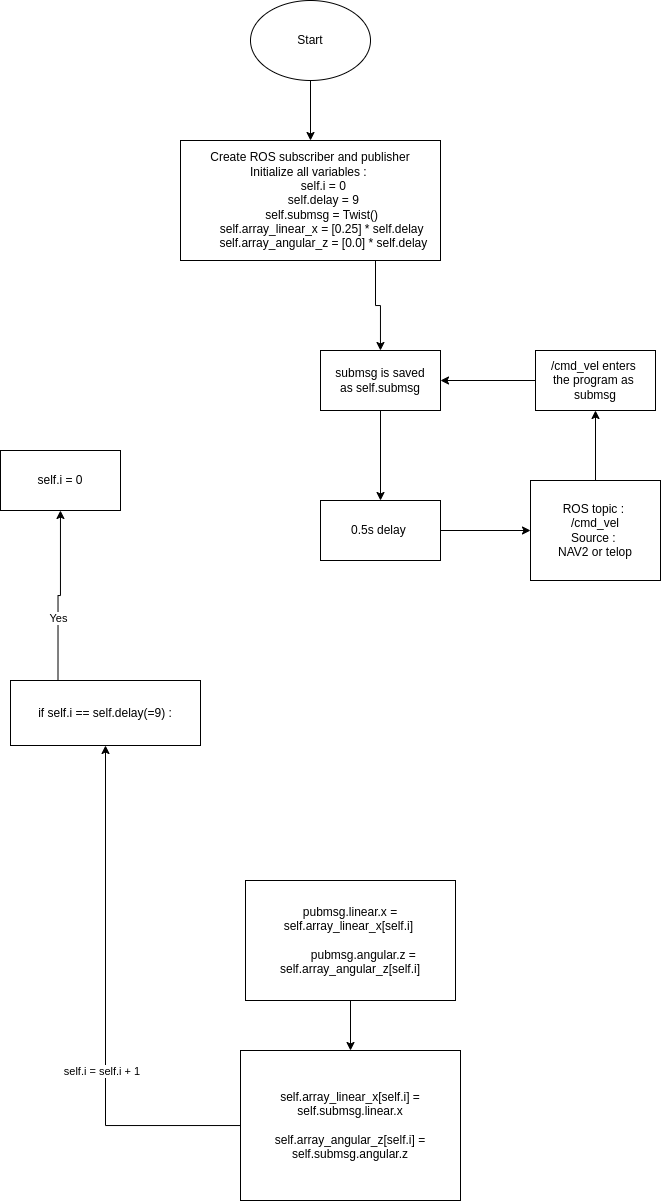
\includegraphics[width = 0.8\textwidth]{Figures/drawio/cmd_vel_subpub.png}
    \caption{Flow chart Time delay algorithm}
    \label{fig:TimeDelayFlow}
\end{figure}

This algorithm where set up and tested and proved to be imprecise. Even though the two vehicles get the same velocity command errors accumulate over time causing the follower to drift of the path. 

\paragraph{Nav2 API} was initiated but remained unfinished due to time constraints. This method is based on the Nav2 API and the fact that the TB3 and the Husky have been setup with the ability to drive autonomously independently. For better understanding here is a list of some Nav2 API commands.

\begin{table}[H]
    \centering
    \begin{tabular}{c|c}
        Command             & Description \\ \hline
        setInitialPose()    & Setting initial pose of a robot \\
        goToPose()          & Publishes a Nav2 Goal \\
        goThroughPoses()    & Publishes a list of Nav2 Goals \\
        getPath()           & Receives the complete ongoing path \\
        changeMap()         & Changes current map to chosen one \\
        getFeedback() & Info about the robot running Nav2 like Time stamp, frame\_id and pose\\
    \end{tabular}
    \caption{Some Nav2 API commands\cite{rosnavAPI}}
    \label{tab:Nav2API}
\end{table}

The idea was both husky and TurtleBot3 run Nav2, a node receives "getFeedback()" from Husky and sends "goToPose()" x distance behind the Husky to the TB3. This task was started on but not finished here is a list with status of the milestones \ref{tab:MilestonesNav2API}.

\begin{table}[H]
    \centering
    \begin{tabular}{c|c}
        Task                                                        & Status   \\ \hline
        Husky driving autonomously with Nav2                        & Complete \\
        TB3 driving autonomously with Nav2                          & Complete \\
        Control Nav2 with API from python                           & Complete \\
        Husky with namespace                                        & Not complete \\
        TB3 with namespace                                          & Complete \\
        Running Nav2 on Husky with namespace                        & Not complete \\
        Running Nav2 on TB3 with namespace                          & Not complete \\
        Running Husky and TB3 on same network with independent Nav2 & Not complete\\
        Node receiving position from Husky and sending goal to TB3  & Not complete \\
    \end{tabular}
    \caption{Milestones of Nav2 API}
    \label{tab:MilestonesNav2API}
\end{table}
   

